\section{Retrieval-augmented generation}
\subsection{In-context learning}
In-context learning is an emergent behavior of Large Language Models that allows them to perform various tasks based on a few input-output examples, without optimizing any parameters. This phenomenon has been observed in LLMs such as GPT-2 \cite{radford2019language} and GPT-3 \cite{NEURIPS2020_1457c0d6}, which have been pre-trained on massive text corpora using a simple objective of predicting the next token given the preceding text. In-context learning relies on the ability of LLMs to store and access factual knowledge in their parameters, and to adapt to different input distributions and output formats by conditioning on the prompt. 
% However, the effectiveness of in-context learning is heavily dependent on the quality and quantity of the examples, and the LLMs may still suffer from poor generalization, catastrophic forgetting, and hallucination issues 4.
\subsection{Information retrieval}

Information retrieval (IR) is the task of finding relevant information from a large collection of documents given a query. IR is an essential component for many NLP applications, such as question answering, dialogue systems. Traditionally, IR methods rely on sparse representations and term-matching techniques, such as TF-IDF \cite{ref1} and BM25 \cite{Amati2009}, to rank documents based on their similarity to the query. However, these methods have limitations in capturing semantic and contextual information, and may fail to retrieve relevant documents that do not share common words with the query.\\\\
To overcome these limitations, recent works have explored the use of dense representations and neural models for IR. In particular, three types of neural architectures based on pre-trained transformer models with the same architecture of BERT \cite{devlin-etal-2019-bert} have been proposed: Bi-encoder, Cross-encoder, and Poly-encoder \cite{Humeau2020Poly-encoders:}. Bi-encoder is efficient and scalable, as it can index and compare the encoded documents using cosine similarity. However, it may not capture the fine-grained interactions between the query and the document. In cross-encoder,  the query and the document are concatenated and passed to a cross-encoder model, which produces a relevance score as the output. Cross-encoder is more accurate and expressive, as it can perform full attention over the query and the document. However, it is slow and impractical, as it has to recompute the encoding for each query-document pair. Poly-encoder combines the advantages of bi-encoder and cross-encoder models by using two separate model, one for the query and one for the document, and applying attention between them only at the top layer. Poly-encoder can achieve better performance than bi-encoder and faster speed than cross-encoder.


\subsection{Unifying retriever and Large Language Model}

One of the challenges of knowledge-intensive tasks, such as open-domain question answering and fact-based text generation, is how to access and integrate external knowledge sources with LLMs. A common approach is to use a two-stage pipeline, where the first stage is a retriever that selects relevant documents or passages from a large corpus, such as Wikipedia, and the second stage is a reader or a generator that produces the answer or the text based on the retrieved information illustrated in Figure \ref{fig:rag}.\\\\
\begin{figure}[hbt]
    \centering
    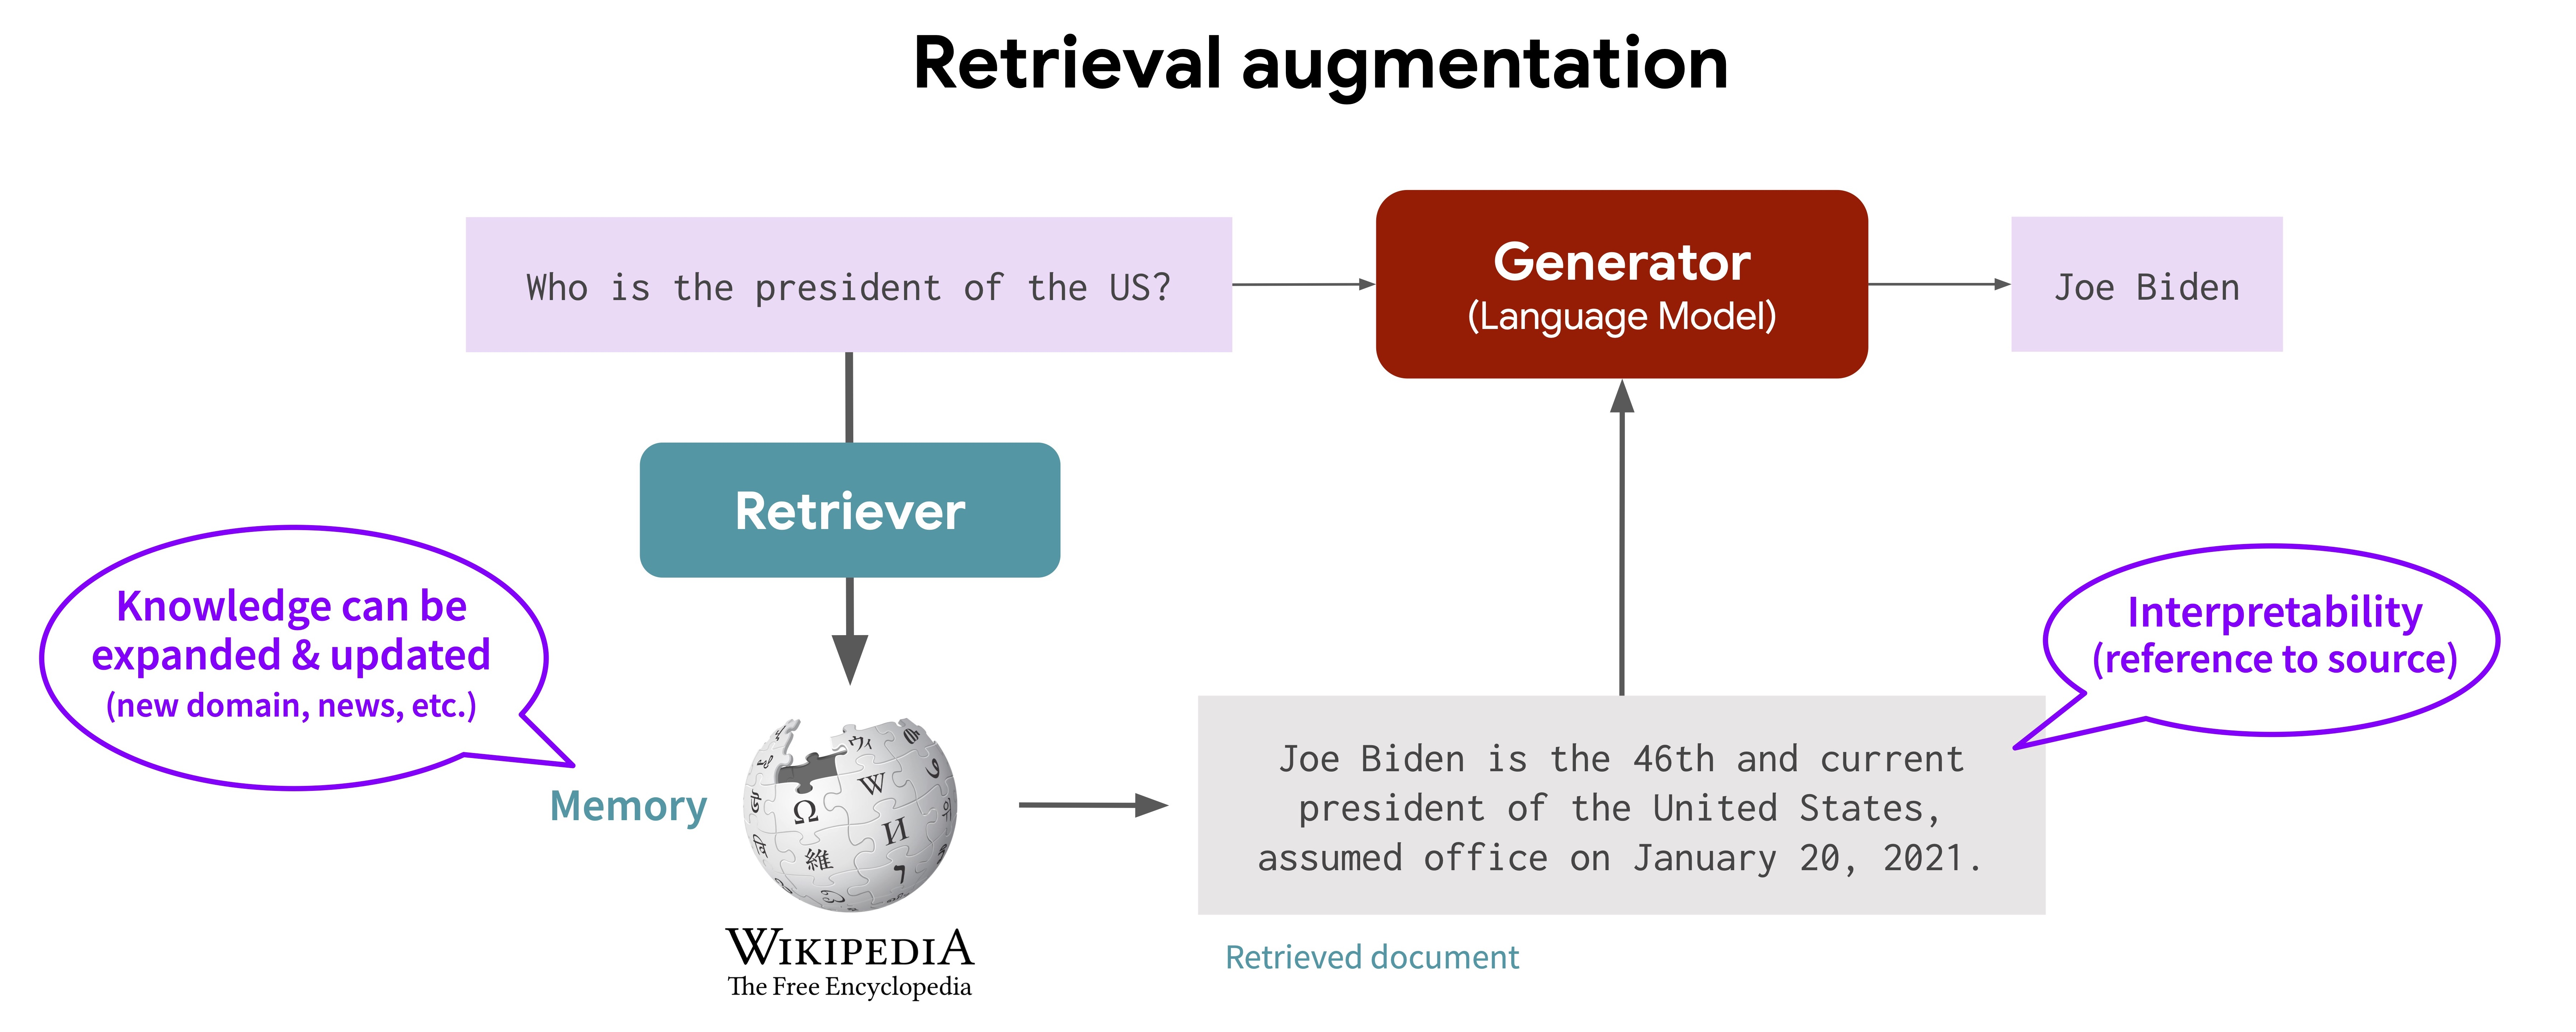
\includegraphics[width=0.8\textwidth]{related-work/images/rag.png}
    \caption{Illustration of two-stage pipeline in retrieval-augmented generation}
    \label{fig:rag}
\end{figure}
A recent line of work \cite{lewis2020retrieval} has proposed to unify the retriever and the LLM in a single end-to-end model, which can jointly learn to retrieve and generate, which combines a pre-trained language model (PLM), BART, with a Dense Passage Retriever (DPR) following the Bi-encoder architecture. This model can use the input sequence to retrieve relevant passages from Wikipedia and use them as additional context when generating the output sequence.
